\section{Code design and implementation}
\label{sec:code}
\begin{figure}
  \begin{center}
    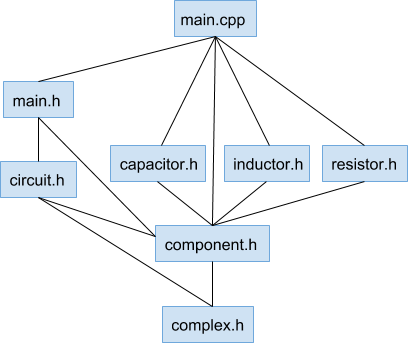
\includegraphics[width=.5\textwidth]{hierarchy}
  \end{center}
  \caption{The hierarchy of header files showing the main file at the top and the chain of its dependencies leading down.}
  \label{fig:hierarchy}
\end{figure}
In the design of this project, the code was split into seven header files, the hierarchical structure of which is shown in figure~\ref{fig:hierarchy}. These header files contained class definitions, function prototypes and a namespace definition while the implementation of the classes, the full functions and the \verb!main! function were separated into seven source files in line with the practice of abstraction, whereby the user is only exposed to the parts of the program which they need to actually use the program, and the details like the member data are hidden from them.

Splitting the code into several files makes it easier to reuse code and limits the \verb!#include! preprocessor directives to what is required only for the small piece of code in the file, and not for the entire program, which reduces the risk of name clashes. Separating into different files can also reduce the compile time, as only the parts that have been changed need to be recompiled and the other object files can just be linked by the compiler.

Header guards were put in place to avoid header files being included multiple times. By using the preprocessor directives to define a unique constant for each header file, the compiler could check using a single if statement whether the header had already been included. This avoids compiler errors caused by apparent redefinitions of existing functions and other problems.

A custom complex class, designed for assignment four of Object Oriented Programming was used for dealing with complex numbers instead of using the standard library type definition. The class contained member data of the type double to store the real and imaginary parts and member functions including functions to calculate the modulus and argument of a complex number, and also defined the division of two complex numbers, all of which were used in the calculation of the impedance and the phase difference.

\renewcommand{\lstlistingname}{Code snippet}

For the components, an abstract base class \verb!Component! was created, from which three derived classes inherited: \verb!Resistor!, \verb!Capacitor! and \verb!Inductor!. The component class defined the functions that the three derived classes had in common -- for instance functions to access and modify the label of the components and a general constructor which was called by the derived classes. The component class had a pure virtual function \verb!get_impedance()! which was then defined in the derived classes, using the functions discussed in section~\ref{sec:theory}. This meant that polymorphic vectors of base class pointers could be created, which could hold resistors, capacitors and inductors. Due to the virtual function in the component class, the three derived classes share a common interface. In this way the same function makes a different calculation depending on what type of object it was called on.

An abstract base class was created for the circuits which was similar to the component base class in that it virtual functions as a shared interface for the \verb!Series! and \verb!parallel! derived classes. Again, the function to calculate the total impedance was left as a pure virtual function in the base class, to be defined according to the equations discussed in section~\ref{sec:theory} within the series and parallel classes. Another virtual function in the \verb!Circuit! class was a function to print the circuit diagram. This was defined separately in the series and parallel classes so that the circuit diagram could be printed in the correct layout for the circuit type.

A library of components was made from which components could be connected in specified groups to create circuits. A similar functionality was added for all circuits that had been made so that circuits from the circuit library could be nested inside other circuits. This was acheived by making two polymorphic vectors of base class pointers -- one for components and the other for circuits. These polymorphic vectors were put inside the namespace \verb!libs! in \verb!main.h! so that the libraries could be accessed from any function using the namespace and the binary scope operator (\verb!libs::!). If the libraries were used multiple times in the same function, \verb!using namespace libs! could be used once to remove the need to type the namespace and binary scope operator repeatedly within the same function.

To ensure that the label of components and circuits is always unique, static member data was used to keep track of the number of each type of component had been added so far. This is private member data which can be accessed by any object created from the class. By inrementing this integer in the constructor, the number of components could be used to create unique labels.

Smart pointers are template classes defined in the \verb!memory! header in the \CC{}11 standard which can be used like pointers and which take care of memory allocation automatically. By instantiating a pointer using \verb!shared_ptr<T>! a pointer of type \verb!T! is created which can be copied and therefore can be owned by multiple entities, for instance different circuits. The advantage of these pointers is that the data stored in the memory address pointed to by \verb!shared_ptr! is deleted automatically when the data goes out of scope. Smart pointers were not implemented in this project as \verb!dynamic_cast()! cannot compare a smart pointer and a pointer, and this function was key in printing the circuit diagrams. An iterator was used to loop through the polymorphic vector of components their symbols, labels and the magnitude of their impedances were printed. When a base class pointer is dynamically cast to a derived class, if the object stored in the memory pointed to by the base class pointer is not the same as the derived class, the dynamic cast returns a null pointer. In this way, the components of the circuit were classified and the relevant symbol was printed.

Input from the user is taken at multiple points in the file, each time with an input to different data types with different allowed values to be input. To avoid having to repeatedly type out checks for the correct input each time the user enters input, a template function \verb!take_input()! was created, as shown in code snippet~ref{lst:input}. The function parameters are defined to be an \verb!initializer_list!, from the header \verb!initializer_list!, which means that the function is called with the argument as a comma separated list of allowed values for the input between two curly braces. The type of the elements of the list of arguments defines the type chosen for the template function, so there is no need to call it in the form \verb!take_input<int>({0,1,2})! unless no allowed inputs are specified. When the program takes input from the user, the input is checked using a while loop whose condition is a lambda which iterates through the vector created by the initializer\_list and checks if the input is present in this list of allowed values.
The lambda returns a boolean value which determines whether to ask for input again.
If an empty list is provided the lambda assumes that there is no range on the input and does not ask for input again as long as the type is correct.
Once the user provides valid input, the \verb!take_input()! function returns this value.
